% ========================================
%	Header einbinden
% ========================================

\documentclass[bibtotoc,titlepage]{scrartcl}

% Deutsche Spracheinstellungen
\usepackage[ngerman,german]{babel, varioref}
\usepackage[T1]{fontenc}
\usepackage[utf8]{inputenc}

%\usepackage{marvosym}

\usepackage{amsfonts}
\usepackage{amssymb}
\usepackage{amsmath}
\usepackage{amscd}
\usepackage{amstext}

\usepackage{longtable}

%\usepackage{bibgerm}

\usepackage{footnpag}

\usepackage{ifthen}                 %%% package for conditionals in TeX
\usepackage[amssymb]{SIunits}
%Für textumflossene Bilder und Tablellen
%\usepackage{floatflt} - veraltet

%Für Testzwecke aktivieren, zeigt labels und refs im Text an.
%\usepackage{showkeys}

% Abstand zwischen zwei Absätzen nach DIN (1,5 Zeilen)
% \setlength{\parskip}{1.5ex plus0.5ex minus0.5ex}

% Einrückung am Anfang eines neuen Absatzes nach DIN (keine)
%\setlength{\parindent}{0pt}

% Ränder definieren
% \setlength{\oddsidemargin}{0.3cm}
% \setlength{\textwidth}{15.6cm}

% bessere Bildunterschriften
%\usepackage[center]{caption2}


% Problemlösungen beim Umgang mit Gleitumgebungen
\usepackage{float}

% Nummeriert bis zur Strukturstufe 3 (also <section>, <subsection> und <subsubsection>)
%\setcounter{secnumdepth}{3}

% Führt das Inhaltsverzeichnis bis zur Strukturstufe 3
%\setcounter{tocdepth}{3}
\usepackage[version=3]{mhchem}
	\mhchemoptions{minus-sidebearing-left=0.06em, minus-sidebearing-right=0.11em}
\usepackage{exscale}

\newenvironment{dsm} {\begin{displaymath}} {\end{displaymath}}
\newenvironment{vars} {\begin{center}\scriptsize} {\normalsize \end{center}}


\newcommand {\en} {\varepsilon_0}               % Epsilon-Null aus der Elektrodynamik
\newcommand {\lap} {\; \mathbf{\Delta}}         % Laplace-Operator
\newcommand {\R} { \mathbb{R} }                 % Menge der reellen Zahlen
\newcommand {\e} { \ \mathbf{e} }               % Eulersche Zahl
\renewcommand {\i} { \mathbf{i} }               % komplexe Zahl i
\newcommand {\N} { \mathbb{N} }                 % Menge der nat. Zahlen
\newcommand {\C} { \mathbb{C} }                 % Menge der kompl. Zahlen
\newcommand {\Z} { \mathbb{Z} }                 % Menge der kompl. Zahlen
\newcommand {\limi}[1]{\lim_{#1 \rightarrow \infty}} % Limes unendlich
\newcommand {\sumi}[1]{\sum_{#1=0}^\infty}
\newcommand {\rot} {\; \mathrm{rot} \,}         % Rotation
\newcommand {\grad} {\; \mathrm{grad} \,}       % Gradient
\newcommand {\dive} {\; \mathrm{div} \,}        % Divergenz
\newcommand {\dx} {\; \mathrm{d} }              % Differential d
\newcommand {\cotanh} {\; \mathrm{cotanh} \,}   %Cotangenshyperbolicus
\newcommand {\asinh} {\; \mathrm{areasinh} \,}  %Area-Sinus-Hyp.
\newcommand {\acosh} {\; \mathrm{areacosh} \,}  %Area-Cosinus-H.
\newcommand {\atanh} {\; \mathrm{areatanh} \,}  %Area Tangens-H.
\newcommand {\acoth} {\; \mathrm{areacoth} \,}  % Area-cotangens
\newcommand {\Sp} {\; \mathrm{Sp} \,}
\newcommand {\mbe} {\stackrel{\text{!}}{=}}     %Must Be Equal
\newcommand{\qed} { \hfill $\square$\\}
\renewcommand{\i} {\imath}
\def\captionsngerman{\def\figurename{\textbf{Abb.}}}

%%%%%%%%%%%%%%%%%%%%%%%%%%%%%%%%%%%%%%%%%%%%%%%%%%%%%%%%%%%%%%%%%%%%%%%%%%%%
% SWITCH FOR PDFLATEX or LATEX
%%%%%%%%%%%%%%%%%%%%%%%%%%%%%%%%%%%%%%%%%%%%%%%%%%%%%%%%%%%%%%%%%%%%%%%%%%%%
%%%
\ifx\pdfoutput\undefined %%%%%%%%%%%%%%%%%%%%%%%%%%%%%%%%%%%%%%%%% LATEX %%%
%%%
\usepackage[dvips]{graphicx}       %%% graphics for dvips
\DeclareGraphicsExtensions{.eps,.ps}   %%% standard extension for included graphics
\usepackage[ps2pdf]{thumbpdf}      %%% thumbnails for ps2pdf
\usepackage[ps2pdf,                %%% hyper-references for ps2pdf
bookmarks=true,%                   %%% generate bookmarks ...
bookmarksnumbered=true,%           %%% ... with numbers
hypertexnames=false,%              %%% needed for correct links to figures !!!
breaklinks=true,%                  %%% breaks lines, but links are very small
linkbordercolor={0 0 1},%          %%% blue frames around links
pdfborder={0 0 112.0}]{hyperref}%  %%% border-width of frames
%                                      will be multiplied with 0.009 by ps2pdf
%
\hypersetup{ pdfauthor   = {Hannes Franke; Julius Tilly},
pdftitle    = {V301 Innenwiderstand und Leistungsanpassung}, pdfsubject  = {Protokoll FP}, pdfkeywords = {V301, Innenwiderstand, Leistungsanpassung},
pdfcreator  = {LaTeX with hyperref package}, pdfproducer = {dvips
+ ps2pdf} }
%%%
\else %%%%%%%%%%%%%%%%%%%%%%%%%%%%%%%%%%%%%%%%%%%%%%%%%%%%%%%%%% PDFLATEX %%%
%%%
\usepackage[pdftex]{graphicx}      %%% graphics for pdfLaTeX
\DeclareGraphicsExtensions{.pdf}   %%% standard extension for included graphics
\usepackage[pdftex]{thumbpdf}      %%% thumbnails for pdflatex
\usepackage[pdftex,                %%% hyper-references for pdflatex
bookmarks=true,%                   %%% generate bookmarks ...
bookmarksnumbered=true,%           %%% ... with numbers
hypertexnames=false,%              %%% needed for correct links to figures !!!
breaklinks=true,%                  %%% break links if exceeding a single line
linkbordercolor={0 0 1},
linktocpage]{hyperref} %%% blue frames around links
%                                  %%% pdfborder={0 0 1} is the default
\hypersetup{
pdftitle    = {V301 Innenwiderstand und Leistungsanpassung}, 
pdfsubject  = {Protokoll AP}, 
pdfkeywords = {V301, Innenwiderstand, Leistungsanpassung},
pdfsubject  = {Protokoll AP},
pdfkeywords = {V301, Innenwiderstand, Leistungsanpassung}}
%                                  %%% pdfcreator, pdfproducer,
%                                      and CreationDate are automatically set
%                                      by pdflatex !!!
\pdfadjustspacing=1                %%% force LaTeX-like character spacing
\usepackage{epstopdf}
%
\fi %%%%%%%%%%%%%%%%%%%%%%%%%%%%%%%%%%%%%%%%%%%%%%%%%%% END OF CONDITION %%%
%%%%%%%%%%%%%%%%%%%%%%%%%%%%%%%%%%%%%%%%%%%%%%%%%%%%%%%%%%%%%%%%%%%%%%%%%%%%
% seitliche Tabellen und Abbildungen
%\usepackage{rotating}
\usepackage{ae}
\usepackage{
  array,
  booktabs,
  dcolumn
}
\makeatletter 
  \renewenvironment{figure}[1][] {% 
    \ifthenelse{\equal{#1}{}}{% 
      \@float{figure} 
    }{% 
      \@float{figure}[#1]% 
    }% 
    \centering 
  }{% 
    \end@float 
  } 
  \makeatother 


  \makeatletter 
  \renewenvironment{table}[1][] {% 
    \ifthenelse{\equal{#1}{}}{% 
      \@float{table} 
    }{% 
      \@float{table}[#1]% 
    }% 
    \centering 
  }{% 
    \end@float 
  } 
  \makeatother 
%\usepackage{listings}
%\lstloadlanguages{[Visual]Basic}
%\allowdisplaybreaks[1]
%\usepackage{hycap}
%\usepackage{fancyunits}


% ========================================
%	Angaben für das Titelblatt
% ========================================

\title{Versuch 101 - Das Trägheitsmoment\\				% Titel des Versuchs 
\large TU Dortmund, Fakultät Physik\\ 
\normalsize Anfänger-Praktikum}

\author{Jan Adam\\			% Name Praktikumspartner A
{\small \href{jan.adam@tu-dortmund.de}{jan.adam@tu-dortmund.de}}	% Erzeugt interaktiven einen Link
\and						% um einen weiteren Author hinzuzfügen
Dimitrios Skodras\\					% Name Praktikumspartner B
{\small \href{dimitrios.skodras@tu-dortmund.de}{dimitrios.skodras@tu-dortmund.de}}		% Erzeugt interaktiven einen Link
}
\date{30.April 2013}				% Das Datum der Versuchsdurchführung

% ========================================
%	Das Dokument beginnt
% ========================================

\begin{document}

% ========================================
%	Titelblatt erzeugen
% ========================================

\maketitle					% Jetzt wird die Titelseite erzeugt
\thispagestyle{empty} 				% Weder Kopfzeile noch Fußzeile

% ========================================
%	Der Vorspann
% ========================================

%\newpage					% Wenn Verzeichnisse auf einer neuen Seite beginnen sollen
%\pagestyle{empty}				% Weder Kopf- noch Fußzeile für Verzeichnisse

\tableofcontents

%\newpage					% eine neue Seite
%\thispagestyle{empty}				% Weder Kopf- noch Fußzeile für Verzeichnisse
%\listoffigures					% Abbildungsverzeichnis

%\newpage					% eine neue Seite
%\thispagestyle{empty}				% Weder Kopf- noch Fußzeile für Verzeichnisse
%\listoftables					% Tabellenverzeichnis
\newpage					% eine neue Seite


% ========================================
%	Kapitel
% ========================================

\section{Einleitung}
Im Zuge dieses Experiments wird das Trägheitsmoment von Körpern, sowie einer Holzpuppe in zwei verschiedenen Positionen bestimmt. 
Weiterhin soll der Satz von Steiner geprüft werden.

\section{Theorie}
Charakteristisch für die Dynamik von Rotationsbewegungen sind die Größen Drehmoment $M$, Trägheitsmoment $I$ und Winkelbeschleunigung
$\dot \omega$. Das Trägheitsmoment einer punktförmigen Masse ist durch $I = m\,r^2$ gegeben. $r$ beschreibt hierbei den Abstand des 
Massepunkts zur Drehachse. Bei ausgedehnten Körpern, bei denen sich die Massenelemente um eine feste Achse drehen, werden 
die einzelnen Trägheitsmomente aufsummiert
\begin{align}
 I = \sum_i r^2_i\,m_i.
\end{align}
Bei einer kontinuierlichen Massenverteilung gilt allgemein
\begin{align}
 I = \int r^2 \dx m.
\end{align}
Daher ist das Trägheitsmoment einfacher, symmetrischer Körper leicht bestimmbar, das komplexerer Körper durch Summation einzelner 
Trägheitsmomente. Sofern die Drehachse aber nicht mit einer Achse des betrachteten Körpers übereinstimmt, sondern um eine Strecke $a$ 
parallel zu  ihr verschoben ist, so kann der Satz von Steiner Abhilfe schaffen
\begin{align}
 I = I_s + m \cdot a^2,
\end{align}
wobei $I_s$ das Trägheitsmoment bezüglich der Drehachse durch den Schwerpunkt ist. 

Bei Rotationsbewegungen von Körpern ist das Drehmoment durch $M = \vec{F} \times \vec{r}$ gegeben. Wenn nun ein schwingbarer Körper
durch eine Auslenkung um den Winkel $\varphi$ aus seiner Ruhelage gebracht wird, wirkt eine Feder ein rücktreibendes Drehmoment auf ihn.
Die Schwingungdauer des Körpers $T$ ist durch sein Trägheitsmoment $I$ und die Winkelrichtgröße $D$ gegeben
\begin{align}
 T = 2\pi \sqrt{\frac{I}{D}}.
 \label{eq_periode}
\end{align}
Das Drehmoment ist mit der Winkelrichtgröße über den Auslenkwinkel verknüpft
\begin{align}
 D = \frac{M}{\varphi}.
 \label{eq_winkel}
\end{align}

\section{Durchführung}
In Abbildung \eqref{pic_aufbau} ist der Aufbau skizziert. Der zu untersuchende Körper ist mit einer Feder gekoppelt, deren Winkelrichtgröße
es zu bestimmen gilt. Wenn eine Federwaage senkrecht zum Radius der vom Körper beschriebenen Kreisbahn mit einem Haken an der Stange
in einem bestimmten Abstand $r$ angesetzt wird, kann für eine Auslenkung $\varphi$ eine Kraft $F$ gemessen werden. 
\begin{figure}[H]
 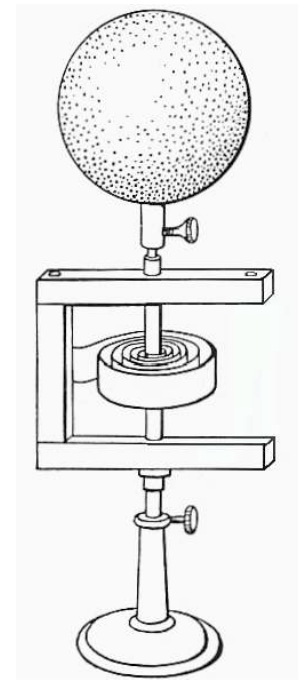
\includegraphics[width=0.3\textwidth]{pics/aufbau.png}
 \caption{Experimenteller Versuchsaufbau$^{[1]}$}
 \label{pic_aufbau}
\end{figure}

Selbst ohne Körper hat die Drillachse ein Eigenträgheitsmoment $I_D$, welches über eine massearme Stange mit zwei Gewichten in Abstand $a$
, welche senkrecht zur Achse angebracht, ermittelt werden kann. Das System, in Schwingung gebracht, oszilliert harmonisch mit einer 
zu messenden Periodendauer $T$. Ohne die Gewichte wird diese wird mittels Stoppuhren über fünf Schwingungsperioden für elf Winkel 
gemessen, woraus der  Mittelwert in die Rechnung eingeht. Mit den Gewichten werden die Schwingungszeiten über je fünf Perioden für 
zehn Abstände $a$ gestoppt. 

Das Trägheitsmoment zweier in Ausdehnungen und Gewicht verschiedener Zylinder wird ebenfalls durch Messung von Periodendauer, sowie 
genannte Ausdehnungen und Masse bestimmt. Die Zeitmessung geschieht analog zu vorangehenden Versuchabschnitten, jedoch lediglich für
fünf Messungen. Ausdehnungen werden mit einer Schieblehre und Massen mit einer Waage bestimmt.

Für eine Holzpuppe soll das Trägheitsmoment in zwei Stellungen (vergleiche Abbildung \ref{pic_puppe}) berechnet werden. Hierbei werden
die einzelnen Bestandteile, heißt Gliedmaßen und Rumpf, als Zylinder angenähert und ihre einzelnen Trägheitsmomente aufsummiert. Ihre 
Ausdehnungen werden an mehreren Stellen gemessen und für die Körperteile jeweils gemittelt. Die Masse ergibt sich dem Produkt von Dichte für Holz
und Volumen aus den Teilvolumina.

\begin{figure}[H]
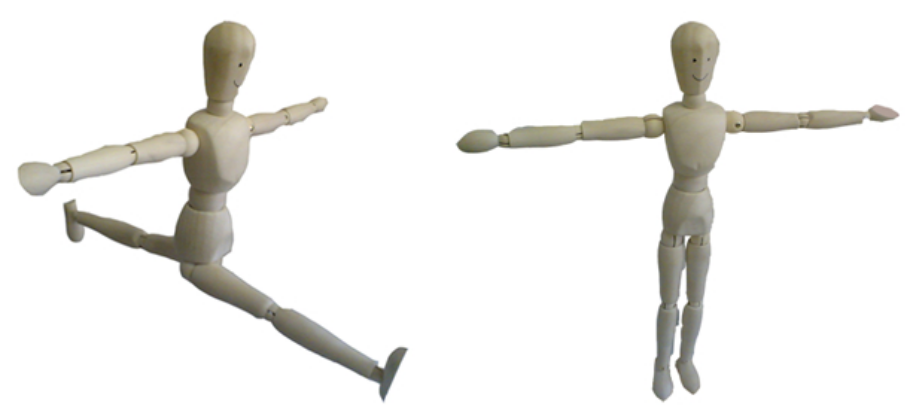
\includegraphics[width=0.8\textwidth]{pics/puppe.png}
\caption{Verwandte Stellungen der Holzpuppe $^{[2]}$}
\label{pic_puppe}
\end{figure}






\section{Auswertung}
\subsection{Winkelrichtgröße und Eigenträgheitsmoment}
Zur Bestimmung der Winkelrichtgröße wird die Feder mit der Querstange daran um verschiedene Winkel ausgelenkt und mittels einer Federwaage die Rückstellkraft bestimmt.\\
Gemessen wurden folgende Werte:
\begin{table}[htbp]
\begin{tabular}{|c|c|}
\hline 
$\varphi$ [Grad]&	F [N]\\ \hline
20	&0,13\\ \hline
40	&0,16\\ \hline
60	&0,21\\ \hline
80	&0,23\\ \hline
100	&0,29\\ \hline
120	&0,34\\ \hline
140	&0,39\\ \hline
160	&0,43\\ \hline
180	&0,48\\ \hline
200	&0,55\\ \hline
220	&0,60\\ \hline
\end{tabular} 
\caption{Messung der Rückstellkraft im Abstand r = 20cm zur Drehachse. Die Winkel wurden relativ groß gewählt, da die Federwaage für kleine Winkel kaum eine Kraft angezeigt hat.}
\end{table}

Mit Gleichung \eqref{eq_winkel} ergibt sich nach einer Umrechnung in Bogenmaß daraus eine Winkelrichtgröße des Aufbaus von:
\begin{align*}
D=(0.035 \pm 0.007) \text{Nm}
\end{align*}


Um Eigenträgheit der Drillachse $I_D$ zu bestimmen, ersetzt man das Trägheitsmoment I in Gleichung \eqref{eq_periode} durch
\begin{align*}
I&=I_D+I_{Stab}+I_{Zylinder} \qquad \text{, wobei}\\
I_{Zyl}&=2m\cdot\left(\frac{R^2}{4}+\frac{l^2}{12}\right)\\
I_{Stab}&= \frac{1}{12}ml^2
\end{align*}
das Trägheitsmoment der beiden Zylinder inklusive dem Betrag durch den Satz von Steiner beschreibt.
Quadriert man die Gleichung und stellt diese um, so erhält man:
\begin{align}
T^2=\frac{8m\pi^2}{D}\cdot a^2 + \frac{4\pi}{D}  \left[  I_D+I_{Stab}+2m\left(\frac{R^2}{4}+\frac{l^2}{12}\right)\right]
\end{align}

\begin{table}[htbp]
\begin{tabular}{|c|c|c|c|}
\hline 
 & Gewicht [g] & Länge [cm] & Breite [cm] \\ 
\hline 
Stab & 96,6 & 30,025 & ----- \\ 
\hline 
Gewichte & 223,6 & 3,04 & 3,5 \\ 
\hline 
\end{tabular}\newline
\caption{Ausmaßen und Massen der Apparatur}
\end{table}

\begin{table}[htbp]
\begin{tabular}{|c|c|}
\hline
a [m] &	T [s]\\ \hline
0,02&	10,57\\ \hline
0,04&	11,85\\ \hline
0,06&	13,19\\ \hline
0,08&	15,56\\ \hline
0,10&	17,01\\ \hline
0,12&	19,23\\ \hline
0,14&	21,43\\ \hline
0,16&	23,47\\ \hline
0,18&	25,67\\ \hline
0,20&	28,05\\ \hline
\end{tabular} 
\caption{Schwingungsdauer der schwingenden Massen. Die Zeiten sind bereits zeitlich gemittelt}
\end{table}

Wird nun $T^2$ gegen $a^2$ aufgetrgagen, so erhält man eine Gerade f(x)= mx+b, mit:
\begin{figure}[htbp]
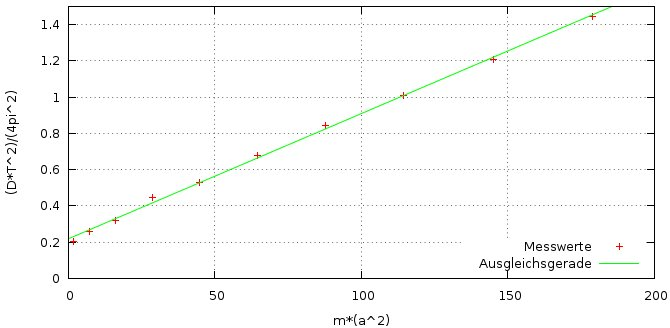
\includegraphics[width=0.8\textwidth]{pics/eigentr.jpg}
\caption{Gemessene Schwingzeit des Systems [s], quadratisch gegen das Quadrat des Abstandes [m] zur Drehachse aufgetragen.}
\end{figure}
\begin{align*}
 m&=\frac{8m\pi^2}{D}=16843,9 \pm 234,6\\
b&=\frac{4\pi}{D}  \left[  I_D+I_{Stab}+2m\left(\frac{R^2}{4}+\frac{l^2}{12}\right)\right]s=118,86 \pm 4,72
\end{align*}

Dadurch kann erstmals das Eigenträgheitsmoment der Drillachse bestimmt werden:
\begin{align*}
I_D=(0,22 \pm 0,07) \text{ kg m$^2$}
\end{align*}

\subsection{Trägheitsmoment zweier Zylinder}
Anschließend wird das Trägheitsmoment zweier Zylinder berechnet und anschließend mit den gemessenen Werten verglichen.

Das Trägheitsmoment eines Zylinders durch seine Symmetrieachse berechnet sich zu:

\begin{align}
I_{Z}=\frac{mR^2}{2}
\label{eq_Izyl}
\end{align}

Die Zylinder haben folgende Daten:
\begin{table}[htbp]
\begin{tabular}{|c|c|c|c|}
\hline 
 & Höhe [m] & Radius [m] & Gewicht [kg]\\ 
\hline 
Zylinder 1 & 0,1008 & 0,0497 & 0,3686 \\ 
\hline 
Zylinder 2 & 0,0302 & 0,0371 & 1,2728 \\ 
\hline 
\end{tabular} 
\caption{Mase der beiden ausgemessenen Zylinder}
\end{table}

Eingesetzt in Gleichung \eqref{eq_Izyl} ergibt dies:
\begin{align*}
I_{Zyl 1}&=(4,54\pm0,0092)\cdot10^{-4}\text{ kg m$^2$}\\
I_{Zyl 2}&=(8,76\pm0,036)\cdot10^{-4}\text{ kg m$^2$}
\end{align*}

Berechnet man das Trägheitsmoment über Gleichung \eqref{eq_periode}, so benötigt man die Schwingzeit der Zylinder:
\begin{table}[htbp]
\begin{tabular}{|c|c|}
\hline 
$t_1$ [s] & $t_2$ [s]\\ \hline
0,74&	1,34\\ \hline
0,73&	1,33\\ \hline
0,76&	1,33\\ \hline
0,74&	1,32\\ \hline
0,75&	1,32\\ \hline
0,73&	1,35\\ \hline
0,73&	1,33\\ \hline
0,75&	1,30\\ \hline
0,73&	1,33\\ \hline
0,74&	1,31\\ \hline
\end{tabular} 
\caption{Schwingungsdauer der zwei vermessenen Zylinder - über fünf Perioden \mbox{gemittelt}}
\end{table}

Die Werte ergeben:
\begin{align*}
t_{Zyl 1}&=(0,739 \pm 0,010)s\\
I'_{Zyl 1}&=(1,00\pm0,69)\cdot10^{-3}\text{ kg m$^2$}\\
\end{align*}
\begin{align*}
t_{Zyl 2}&=(1,325 \pm  0,014)s\\ 
I'_{Zyl 2}&=(3,22\pm5,86)\cdot10^{-3}\text{ kg m$^2$}
\end{align*}

\subsection{Trägheitsmoment einer Puppe}
Zum Schluss soll das Trägheitsmoment einer Puppe bestimmt werden. Die Gliedmaßen werden dabei als Zylinder angenährt und ihr Umfang wird an ungefähr 10 verschiedenen Stellen gemessen, um einen präzisen Mittelwert zu erhalten.

Folgende Tabelle beinhaltet alle gemessenen Größen:
\begin{table}[H]
\begin{tabular}{|c|c|c|c|}
\hline 
Bein&	Arm	&Oberk	&Kopf	\\ \hline
1.79&	1.69&	3.49&	1.44\\ \hline
2.13&	1.58&	4.06&	1.55\\ \hline
1.90&	1.64&	3.76&	1.89\\ \hline
1.71&	1.50&	3.37&	2.38\\ \hline
1.62&	1.35&	3.02&	2.55\\ \hline
1.29&	1.11&	2.53&	2.79\\ \hline
1.69&	1.39&	2.56&	2.95\\ \hline
1.63&	1.51&	2.97&	3.07\\ \hline
1.36&	1.26&	3.64&	2.51\\ \hline
1.31&	1.00&	3.97&		\\ \hline
	&	3.89&		&		\\ \hline
\end{tabular}
\caption{Durchmesser der entsprechenden Körperteilen an verschiedenen Stellen gemessen - die gemittelten Werte d finden sich in den folgenden Tabelle}
\end{table}
\begin{table}[htbp]
\begin{tabular}{|c|c|c|c|c|}
\hline 		
&	Bein&	Arm	&Oberkörper	&Kopf	\\ \hline	
d [cm]&	1,643&	1,40&	3,34&	2,113\\ \hline				
l [cm] &	15,39	&13,80	&10,00	&5,48\\ \hline	
					
V [$\cdot 10^{-6} m^3$]	&32,63	&21,33	&87,46	&19,22	\\ \hline	
Anteil am Gesamtvolumen	&0,203	&0,133	&0,544	&0,120	\\ \hline		
m [g]	&32,66	&21,35	&87,55 &19,24\\ \hline
Abstand [cm]	&2,18	&16,78	&&\\ \hline	
					
I[$\cdot 10^{-6}$kg m$^2$]&		 1,66	&63,55&	1,22	&1,0735\\ \hline	
\end{tabular} 
\caption{Puppe mit ausgestreckten Armen (Position 1)}
\end{table}

Summiert man über alle Teilträgheiten I, so erhält man als Trägheitsmoment der Puppe:
\begin{align*}
I_{Pos 1}= 1,317\cdot 10^{-3}\text{ kg m$^2$}
\end{align*}

\begin{table}[htbp]
\begin{tabular}{|c|c|c|c|c|}
\hline 		
&	Bein&	Arm	&Oberkörper	&Kopf	\\ \hline	
d [cm]	&1,64	&	1,40	&	3,34	&	2,11	\\ \hline		
l [m]	&15,39	&	13,80	&	10,00	&	5,48\\ \hline	
V [$\cdot10^{-6}m^3$]	&32,63	&21,33	&87,46	&19,22\\ \hline	
Anteil am Gesamtvolumen&	0,203	&0,133&	0,544	&0,120\\ \hline
m [g]	&32,66&	21,36	&87,55	&19,24\\ \hline	
Abstand [cm]&	9,36	&16,78&&\\ \hline	
I[$\cdot 10^{-6}$kg m$^2$]&		539,39&	635,46&	12,19&	1,07\\ \hline	
\end{tabular} 
\caption{Puppe mit ausgestreckten Armen und Beinen (Position 2)}
\end{table}

Man erhält als Trägheitsmoment der Puppe:
\begin{align*}
I_{Pos 2}=1,99\cdot 10^{-3}\text{ kg m$^2$}
\end{align*}

Zum Vergleich kann man die Trägheit immer noch nach Gleichung \eqref{eq_periode} berechnen. Man benötigt dazu die Schwingzeiten:
\begin{table}[H]
\begin{tabular}{|c|c|}
\hline 
Position 1 [s] & Position 2 [s]\\ \hline 
2,92&	4,35\\ \hline 
2,89&	4,32\\ \hline 
2,78&	4,21\\ \hline 
2,81&	4,27\\ \hline 
2,84&	4,16\\ \hline 
2,84&	4,28\\ \hline 
2,78&	4,25\\ \hline 
2,87&	4,34\\ \hline 
2,87&	4,19\\ \hline 
2,78&	4,16\\ \hline 
\end{tabular} 
\caption{Gemessene Schwingzeiten in Sekunden für beide Körperhaltungen}
\end{table}

Und erhält damit für die Trägheitsmomente:
\begin{align*}
I'_{Pos 1}=(12,3 \pm 2,9)\cdot 10^{-3} \text{ kg m$^2$}\\
I'_{Pos 2}=(27,7 \pm 6,5)\cdot 10^{-3} \text{ kg m$^2$}
\end{align*}

\section{Diskussion}
Das Eigenträgheitsmoment der Drehachse lässt sich relativ genau berechnen, dagegen weichen die Werte für die Winkelrichtgröße bei kleinen Winkeln stark von dem Ergebnis ab. Dies ist vermutlich darauf zurückzuführen, dass die Apparatur eine relativ hohe Reibung hat, die sich besonders bei kleinen Auslenkungen bemerkbar macht. Die Gleichung gilt jedoch eigentlich nur für kleine Winkel, daher ist die Auswertung über die Federwaage aussagekräftiger, denn bei ihr werden Reibungen nicht berücksichtigt.
\begin{table}[htbp]
\begin{tabular}{|c|c|}
\hline 
$D$ [\text{Nm}]  & $(0,072 \pm0,023)$ \\ \hline 
$I_D[\text{ kg m$^2$}]$ & $(0,22 \pm 0,07)$ \\ \hline 
$I_{Zyl 1}[\text{ kg m$^2$}]$&$(0,454\pm0,001)\cdot10^{-3}$\\ \hline 
$I'_{Zyl 1}[\text{ kg m$^2$}]$&$(1,00\pm0,69)\cdot10^{-3}$\\ \hline 
$I_{Zyl 2}[\text{ kg m$^2$}]$&$(0,876\pm0,004)\cdot10^{-3}$\\ \hline 
$I'_{Zyl 2}[\text{ kg m$^2$}]$&$(3,22\pm5,86)\cdot10^{-3}$\\ \hline 
$I_{Pos1}[\text{ kg m$^2$}]$&$1,317\cdot 10^{-3}$\\ \hline 
$I'_{Pos1}[\text{ kg m$^2$}]$&$(12,3 \pm 2,9)\cdot 10^{-3}$ \\ \hline 
$I_{Pos2}[\text{ kg m$^2$}]$&$1,99\cdot 10^{-3}$\\ \hline 
$I'_{Pos2}[\text{ kg m$^2$}] $&$(27,7 \pm 6,5)\cdot 10^{-3}$\\ \hline 
\end{tabular}
\caption{Alle Ergebnisse des Versuches zusammengestellt. Die gestrichenen Werte sind dabei Ergebnisse aus einer Berechnung über die Schwingzeit.}
\end{table}

Die Trägheitsmomente der beiden Zylinder liegen um einen Faktor von ungefähr 3 auseinander, wenn man die theoretischen mit den gemessenen Werten vergleicht. Auch dies lässt sich vermutlich darauf zurückführen, dass die Apparatur zu stark gedämpft ist. Die Körper schwingen recht schnell und um den statistischen Fehler zu minimieren muss man über mehrere Schwingungen mitteln. Da die Amplitude jedoch um gut 15\% pro Periode abnimmt, schlägt dieser Fehler dann mehr ins Gewicht.

Bei den Trägheitsmomenten der Puppe merkt man den Unterschied zu den Theoriewerten am deutlichsten. Die Werte liegen eine ganze Größenordnung auseinander. Das die Differenz hier besonders groß ist, hat verschiedene Gründe. Zum einen wirkt sich wieder die Dämpfung der Apparatur auf die Messung aus. Zum anderen ist die Figur aber auch nicht genau mittig auf ihrer Symmetrie befestigt und ihre Haltung ist relativ instabil. Lässt man sie Schwingen bewegen sich die Gliedmaßen auf Grund der Fliehkraft automatisch ein wenig nach außen, wodurch sich das Trägheitsmoment ändert.\\
Außerdem ist die Puppe nicht richtig fest auf dem Stab befestigt und rutscht bei größeren Beschleunigungen hin und her.
Bei den Theoriewerten schlägt am härtesten zu Buche, dass die Puppe nur grob aus Zylindern angenährt wurde. Die genaue Mittelung minimiert diesen Fehler zwar, dennoch ist er deutlich zu spüren. Zudem wurden Füße und Hände der Puppe, sowie der Metallstab völlig vernachlässigt.


\parskip 100pt
\Large{Literatur}\\\\
\large{[1] Versuchsanleitung - Das Trägheitsmoment}\\\\
\large{[2] Cauet C. \& Brambach T. (2006), \textit{Protokoll zu Versuch 101 - Trägheitsmomente starrer Körper}, S.4}\\\\

% ========================================
%	Literaturverzeichnis
% ========================================

%\bibliographystyle{plainnat}			% Bibliographie-Style auswählen
%\bibliography{BIBDATEI}			% Literaturverzeichnis

% ========================================
%	Das Dokument endent
% ========================================

\end{document}
